\section{\I{Partition \& Categories}\label{sec:partition-categories-section}}

Dividing the population into different categories is fundamental to modelling the dynamics of a fish stock. CASAL had a fixed set of hard-wired categories (e.g., factors like sex, area, or stock) and each category type had a predefined set of allowed processes (or transitions in CASAL-speak), e.g., immature fish moving into mature category \citep{1388}. This made sense when CASAL was coded, but now it is seen as a limitation, e.g., changing sex was not allowed and there can only be male and female sexes, not an unknown sex that sometimes occurs in data. [TODO: shift to intro or drop?]

In \CNAME\, the concept of user defined categories was introduced to allow more flexibility in dividing up the population. Note that \CNAME\ does not know about sex or area and their properties; these are explicitly built up by the user by specifying processes that act on the categories in the input files. The cost is that users need to follow good practice to achieve clarity and readability of the input files, i.e., poor specifications can result in obscure input files.

\subsection{Specifying the partition using categories}

A key element of the model is the partition which holds the current state of the population. The partition can be conceptualised as a matrix, where each row represents a category and the columns are the age classes (Figure~\ref{Fig:part}). Each row represents all individuals in that category as a numbers-at-age vector.  There must be at least one category defined for each model.

\begin{figure}[H]
	\centering
	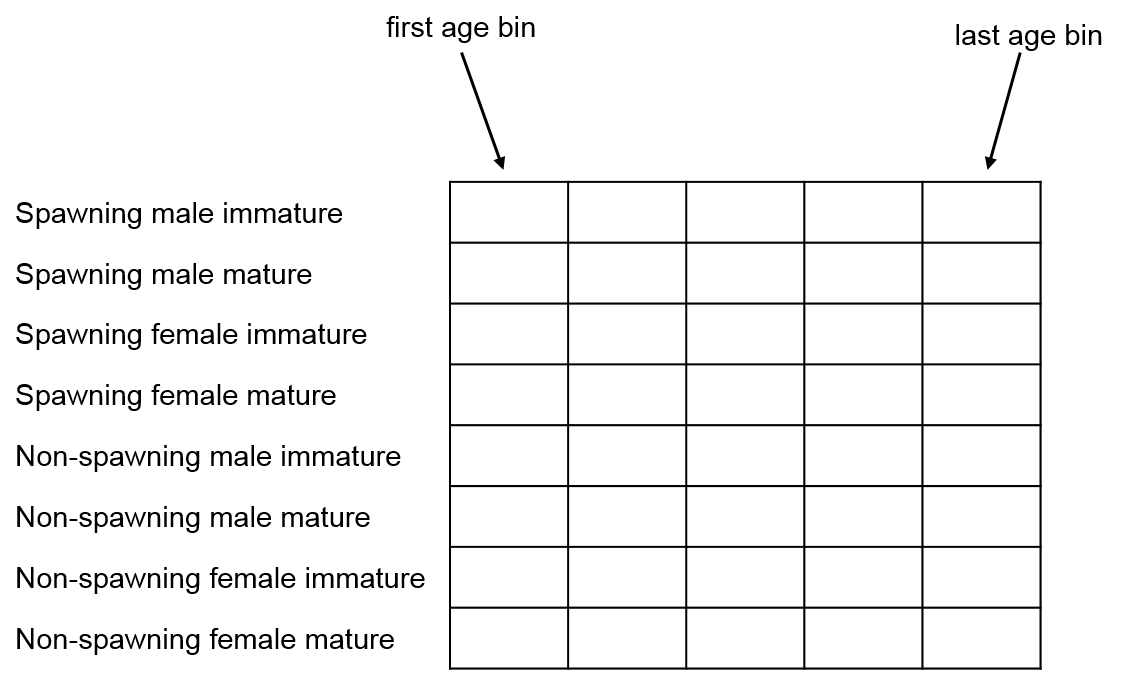
\includegraphics[scale=0.4]{Figures/partition2.png}
		\caption{A visual representation of a partition.}\label{Fig:part}
\end{figure}

The categories can include combinations of levels from one or more factors such as sex, maturity state, area, or even species. \CNAME\ has no predefined categories; \emph{all} categories are defined by the user. Note that the partition only has the current state of the model; past states are not kept (\textit{See} the section on derived quantities about saving past summaries from the partition, p. \pageref{sec:derived-quantities}).

To illustrate categories, consider a model of a fish population with two fisheries, one on spawning fish at the spawning grounds and another on the non-spawning population in the rest of the stock area. The mature fish will migrate to the spawning area, where the spawning fishery occurs. At the end of spawning, these fish, along with the recruits from the previous year, migrate back to the non-spawning area. The fish population can be represented  by factors sex (levels \textit{male} and \textit{female}), maturity (levels \textit{immature} and \textit{mature}), and area (levels \textit{spawning} and \textit{non-spawning} ). So the partition has 8 rows of numbers-at-age, from 2 sexes $\times$ 2 maturity levels $\times$ 2 areas.

These categories are specified in a categories block which starts with a \textit{@categories} line followed on the next line by a \textit{format} subcommand that specifies the factors to use and their order. Factor names are user defined and have no intrinsic meaning to \CNAME). The command block is:

{\small{\begin{lstlisting}
	@categories
	format area.sex.mature
	names spawn.male.immature spawn.male.mature spawn.female.immature spawn.female.mature nonspawn.male.immature nonspawn.male.mature nonspawn.female.immature #all on one line nonspawn.female.mature  
\end{lstlisting}}}  %{verbatimIJD}}}

Note the "." syntax to separate the factor names.

Next comes the \textit{names} subcommand which specifies the combinations of levels that makes up each category. In a sense, the \textit{format} subcommand is not needed since the \textit{names} subcommand can define all categories. However, \textit{format} allows a more  digestible and shorter syntax to define categories here and in other blocks such as matching observation to categories that provided the data (including combinations of categories, e.g., age compositions that combine both sexes).

For example, the \textit{names} subcommand can be specified by:

{\small{\begin{verbatim}names spawn,nonspawn.male,female.immature,mature
\end{verbatim}}}

which defines the categories above in a more efficient manner, (again, note the "." to separate the factors and "," to separate the levels within each factor (\textit{see} the next section for more details). A visualisation of the partition is in Figure \ref{Fig:part}.

When using the short-cut syntax in \textit{names}, the order of level combinations is for the levels of the first factor to change the slowest, then the next factor will change faster, and so on with the last factor to changing levels the fastest. The order is important because linking categories to their characteristics, e.g., growth curve or selectivity, is done in other subcommands where these must be specified in the same order.

To exclude unused categories from the partition, the long form must be used in the \textit{names} subcommand, e.g., to exclude  \textit{spawn.female.immature} and \textit{spawn.male.immature} since they are never in the spawning area.

To make recruitment to enter the partition in  the non-spawning area, use

{\small{\begin{lstlisting}
	@categories
	format area.sex.mature
	names spawn.male.mature spawn.female.mature nonspawn.male.immature nonspawn.male.mature nonspawn.female.immature   
\end{lstlisting}}}

\subsection{Shorthand syntax for categories}\label{sec:ShorthandSyntax-section}

This can be skipped on the first reading.

Some specifications have long lists of categories or years or initial values for parameters and the like, e.g., for YCS from 1900 to 2019, 120 years and 120 initial vales of YCS must be specified; this is hard to do by hand and it can be error prone as well as difficult to match values for each year. Here, the range short cut (\textit{:)} can be used so the  the year specification is \textit{1900:2019}, and the multiplier short cut (\textit{*)} to give the initial values specification as \textit{1*120}.

There is also shorthand notation for categories since each category can be quite complicated. \label{sub:categories}. First use the \texttt{format} subcommand in the \textit{@categories} block to define the factors that make up the sections of the category names. A "." (period) character delineates each factor and this structure allows a shorthand syntax to compose category names. 

The \texttt{names} subcommand is used to list the category names. Sections within the shorthand syntax for \textit{names} are required to match the order of factors in the \textit{format} subcommand so \CNAME\ can organise and search on them. In these sections, levels for each factor use the "list specifier" and range characters, e.g.,

{\small{\begin{lstlisting}
@categories
format sex.stage.tag   # 2 sexes, 2 stages, tag years 2001 to 2005 = 20 categories

names male.immature               # Invalid: No tag information
names female                      # Invalid: no stage of tag information
names female.immature.notag.1    # Invalid: Additional format segment not defined

names male,female.immature,mature.notag,2001:2005 # Valid shortcut

# Without the shorthand syntax these categories would be written:

names male.immature.notag male.immature.2001 male.immature.2002 male.immature.2003 male.immature.2004 male.immature.2005 male.mature.notag male.mature.2001 male.mature.2002 male.mature.2003 male.mature.2004 male.mature.2005 female.immature.notag female.immature.2001 female.immature.2002 female.immature.2003 female.immature.2004 female.immature.2005 female.mature.notag female.mature.2001 female.mature.2002 female.mature.2003 female.mature.2004 female.mature.2005
\end{lstlisting}}}

The shorthand syntax available are: [TODO: edit list]

\begin{itemize}
	\item \textit{*} Specify all categories
	\item \textit{+} Categories join, e.g., \textit{categories *+} joins all categories together into one unit; \textit{categories male+female}
specifies that the observation covers both sexes combined.
    \item \textit{:} Specify a range of integers <int1>:<int2>, e.g., \textit{2000:2005} expands to \textit{2000, 2001, 2002, 2003, 2004, 2005}
    \item Lists using ",": <item1>,<item2>,<item3>, e.g., \textit{male,female,unsexed} are the levels for the factor \textit{sex}.
    \item Repeats a number or label: <number~|~label>*<integer>, e.g., \textit{1*5} --> \textit{1 1 1 1 1} 
    \item \textit{format=<X>=<x>=<int>}   ??? no idea how it works
    \textit{<factor>=level>=<year range>}, e.g., \textit{tag=2001=1999:2003} the categories with level 2001 in the tag factor are accessible from year 1999 to 2003 inclusive, i.e, these categories are not not part of the partition in the years prior to 1999 (saves computation effort). format=??
    \item \textit{[]} replace label to a command block with the block defined inline, e.g., \textit{catchability [q = 1e-5]} rather than \textit{catchability CHATq} where \textit{CHATq} labels a command block somewhere in the input files
\end{itemize}


Example of specifying categories using the short cuts:

This syntax is the long way:
{\small{\begin{verbatim}
		@categories
		format sex.stage
		names male.immature male.mature female.immature female.mature
\end{verbatim}}}

A shorter way to specify the exact same partition structure  using \textit{lists}:

{\small{\begin{verbatim}
		@categories
		format sex.stage
		names male,female.immature,mature
\end{verbatim}}}

\CNAME\ requires categories in processes and observations so that the correct model dynamics can be applied to the correct elements of the partition.

This block illustrates using categories required for the ageing process:

{\small{\begin{verbatim}
		# 1. The long-hand way
		@ageing my_ageing
		categories male.immature male.mature female.immature female.mature

		# 2. The first shorthand way
		@ageing my_ageing
		categories male,female.immature,mature

		# 3. Wild Card (all categories)
		@ageing my_ageing
		categories *

		# 4. The second shorthand way (\textit{obscure}
		@ageing my_ageing
		categories sex=male sex=female
\end{verbatim}}}

To combine/aggregate categories together, use the "\texttt{+}" special character. For example, this feature can be used to specify that the total biomass of the population is made up of both males and females.

For example,

{\small{\begin{verbatim}
		@observation CPUE
		type biomass   # observation using an index of biomass
		categories male+female
        ...   # other subcommands to link index to the fishery etc
\end{verbatim}}}

This combination/aggregation functionality can be used to compare an observation to the total combined population:

{\small{\begin{verbatim}
		@observation CPUE
		type biomass
		categories *+
 ...   # other subcommands to link index to the fishery etc
		\end{verbatim}}}

If the levels \subcommand{male} and \subcommand{female} are the only categories in a population (i.e., factor sex), then this is the same syntax as the command block above it.

Shorthand syntax can be useful when applying processes to a select group of categories from the partition.

For example, to apply a spawning migration to the mature categories in the partition giving the partition definition:

{\small{\begin{verbatim}
		@categories
		format area.maturity.tag
		names north,south.immature,mature.notag,2001:2005
\end{verbatim}}}

Then, to migrate a portion of the mature population from the southern area to the northern area:

{\small{\begin{verbatim}
		@process spawn_migration
		type transition_category   #process to move fish from one category to another
		from format=south.mature.* #move all south mature fish, both notag and tagged fish  
		to format=north.mature.*   # into the relevant north categories
\end{verbatim}}}

\textbf{Advanced partition syntax}

Specific data for a year in a category can be set up so that this category is not to be processed during specific years or in the initialisation phases. Years that each category is available can be specified and these years which will override the default setting of all years in the model. Any category with the default years overridden will no longer be accessible in the initialisation phases.

Examples:

{\small{\begin{verbatim}
@model
start_year 1998   #the model starts in 1996 and
final_year 2010   # goes through to 2010

@categories
format sex.stage.tag
names male,female.immature,mature.notag,2001:2005 # Valid
# Specify categories with the tag value "2001" are available in years 
        #1999, 2000, 2001, 2002, 2003
# And also for categories with the tag value "2005" are available in years 
        #2003, 2004, 2005, 2006, 2007
years tag=2001=1999:2003  tag=2005=2003:2007
\end{verbatim}}}
%\label{sec:ShorthandSyntax-section}
%\resizebox{\textwidth}{!}{%

\begin{table}[h]
\tiny
\center
\begin{tabular}{lrrrrrr}
Category&\multicolumn{5}{r}{Age} &names syntax fragment\\
\cline{2-6}
&1&2&3&4&5\\
\hline
male.immature&0&0&0&0&0&male,female.immature,mature\\
male.mature&0&0&0&0&0\\
female.immature&0&0&0&0&0\\
female.mature&0&0&0&0&0\\
male.immature.2005&0&0&0&0&0&male,female.immature,mature.2005:2010\\
male.immature.2006&0&0&0&0&0\\
male.immature.2007&0&0&0&0&0\\
male.immature.2008&0&0&0&0&0\\
male.immature.2009&0&0&0&0&0\\
male.immature.2010&0&0&0&0&0\\
male.mature.2005&0&0&0&0&0\\
male.mature.2006&0&0&0&0&0\\
male.mature.2007&0&0&0&0&0\\
male.mature.2008&0&0&0&0&0\\
male.mature.2009&0&0&0&0&0\\
male.mature.2010&0&0&0&0&0\\
female.immature.2005&0&0&0&0&0\\
female.immature.2006&0&0&0&0&0\\
female.immature.2007&0&0&0&0&0\\
female.immature.2008&0&0&0&0&0\\
female.immature.2009&0&0&0&0&0\\
female.immature.2010&0&0&0&0&0\\
female.mature.2005&0&0&0&0&0\\
female.mature.2006&0&0&0&0&0\\
female.mature.2007&0&0&0&0&0\\
female.mature.2008&0&0&0&0&0\\
female.mature.2009&0&0&0&0&0\\
female.mature.2010&0&0&0&0&0\\
unsexed.immature&0&0&0&0&0&unsexed.immature\\
  \end{tabular}
  \caption{Partition using: \textit{names male,female.immature,mature  male,female.immature,mature.2005:2010  unsexed.immature} }\label{Tab:part}
\end{table}

Category shortcuts can be used in a sequence to create a complex partition. For example, using the following creates the partition shown in Table \ref{Tab:part}.

{\small{\begin{lstlisting}
@categories
format sex.maturation.tag
names male,female.immature,mature male,female.immature,mature.2005-2010 unsexed.immature 
#<is equal to>
names male.immature male.mature female.immature female.mature
      male.immature.2005 male.immature.2006 male.immature.2007 male.immature.2008 male.immature.2009 male.immature.2010
      male.mature.2005 male.mature.2006 male.mature.2007 male.mature.2008 male.mature.2009 male.mature.2010
      female.immature.2005 female.immature.2006 female.immature.2007 female.immature.2008 female.immature.2009 female.immature.2010
      female.mature.2005 female.mature.2006 female.mature.2007 female.mature.2008 female.mature.2009 female.mature.2010      
      unsexed.immature
\end{lstlisting}}}

Note that the algorithm goes from left to right over the factors in the \textit{format} subcommand. So substituting \textit{unsexed} for \textit{unsexed.immature} is valid and gives a category called \textit{unsexed} in the \textit{sex} factor. But substituting \textit{.immature} (or \textit{.zzz}) for \textit{unsexed.immature} results in one less category and generates an error (i.e., no level provided for factor \textit{sex}).

\subsection{\I{Referencing vector and map parameters}\label{sec:params}}

TODO: has ref been done above?? shift? or new sction?

To build relationships between command blocks, \CNAME\ uses  a referencing system so that blocks and parameters within blocks can be accessed. In its simplest form, command blocks are referenced by their label. To access specified parameters within a command block, the syntax used is:

{\small{\begin{verbatim}
<syntactic element>     #<>  enclosing a description of the element

<block type>[<label of block>].<parameter name>         # most used version
<block type>[<label of block>].method_<parameter name>  #e.g., identify a  fishery

#Examples
process[recruitment].ycs         #ycs parameter in the process block called recruitment
process[Fishing].m               #natural mortality in the process called Fishing

process[Fishing].method_pot      #pot fishery in the process called Fishing
                                 # it is usual to define all fisheries in one 
                                 # mortality process block so we need a way to
                                 # identify each one
\end{verbatim}}}

Parameters can be scalars (one value), vectors (several values), or maps. A map consists of two vectors: one containing a key value (for searching or uniquely indexing), and another vector that contains values associated with the index, e.g., specifying YCS values for each year; the years are the key (or index). To reference one or more components of a vector or map use the \textit{\{\}} syntax. This is sometime needed when specifying which element(s) in a vector or map are to be estimated.

An example of a map parameter is \texttt{ycs\_values} in a recruitment process

{\small{\begin{verbatim}
		@process   WestRecruitment
		type       recruitment_beverton_holt  # Beverton-Holt function
		ycs_values 1 1 1 1 1 1 1 1      # initial values of the YCS (a vector with 9 values)
		ycs_years 1975:1983             #key into YCS
		# An alternative method to specify a sequence of values
		# use an asterisks to represent a vector of repeating integers
		ycs_values 1*8
\end{verbatim}}}

To specify that only the last four years of the YCS parameter \texttt{process[WestRecruitment].ycs\_values} are to be  estimated:

{\small{\begin{verbatim}
		@estimate YCS    #YCS is a label to identify this block
		parameter process[WestRecruitment].ycs_values{1980:1983}  #estimate 4 values only: 1980 1981 1982 & 1983
\end{verbatim}}}

To estimate a common value for a block of years in a map parameter use the \textit{same} subcommand. We illustrate the idea within the process \command{time\_varying}\texttt{[label].type=constant}, where we want to fix \textit{q} over a specified block of years, 1992 to 1995.

First specify the relationships in a \command{time\_varying} block:

{\small{\begin{verbatim}
		@time_varying q_step1
		type          constant                #specify a set value for a year
		parameter     catchability[Fishq].q   # parameter ref for q in block Fishq
		years 	1992	1993	1994	1995  #or 1992:1995 = key into value
		value 	0.2		0.2		0.2		0.2   # or 0.2*4, initial values of q
\end{verbatim}}}

Next, to estimate only one \textit{q} value for the time block, pick one element of the map (say 1992), and then force all other years to have the same value:

{\small{\begin{verbatim}
		@estimate q_block_1992
		parameter time_varying[q_step1].value{1992}  #estimate this one
		same      time_varying[q_step1].value{1993:1995}  #set these to the value for 1992
		type      uniform                   #uniform prior on q
		lower_bound 0.1 
		upper_bound  10  
\end{verbatim}}}

Keys are restricted in \CNAME\ to years and categories. An example using categories as a key in a map:

{\small{\begin{verbatim}
@category
factor sex
names male female

@process recruit
categories male female   #key for m
m  0.17 0.17             # natural mortality values indexed by categories
...

@estimate M
type uniform                     #prior
parameter recruitment.[m]{male}  # estimate male M, "male" is a level for factor sex
same recruitment.[m]{female}     # set female M to the same value as male's
\end{verbatim}}}
	
For vector parameters (i.e., no key values), the index is an integer starting with 1 for the first value. An example is the selectivity \textit{all.values.bounded} which can be defined by:

{\small{\begin{verbatim}
@selectivity MatSel
type         all_values_bounded
L            2              #lower bound at age 2
H            4              # upper bound at age 4
v            0.1 0.2 0.7   # 3 values, one for each age 2, 3, and 4

@estimate  mature
type       uniform                   #prior
parameter selectivity[MatSel].v{2}  # estimate the 2nd value only, i.e., age 3
lower_bound 0.1                     # lower parameter range
upper_bound 1.0                     # upper parameter range
\end{verbatim}}}
	
The integer \textit{{2}} cannot be used to specify the \textit{q} parameter for 1993 in the above example labeled \textit{q\_block\_1992}. This will pass the syntax test, but it will fail at the validate stage in \CNAME.


\paragraph*{\I{In-line declaration, avoiding extra command blocks}\label{sec:declare}}

In-line declarations can help shorten models by defining \command{} blocks within the subcommand line instead of having a label that points to a command block define somewhere else in the input files.

For example, catchability for an CPUE index series can be defined inline:

{\small{\begin{verbatim}
		@observation chatCPUE
		type biomass                   # biomass index
		catchability [q=6.52606e-005]  # define catchability here
		categories male+female         # index cover both sexes together


		@estimate chatCPUE_q
		parameter catchability[chatTANbiomass.one].q #how to reference q
		type uniform_log     # prior
		lower_bound 1e-2
		upper_bound 1
		\end{verbatim}}}

In the above code catchability is defined and estimated without explicitly creating a \command{catchability} block.

\subsection{Examples? not needed?}

